\documentclass[working, oneside]{inputs/tuftebook}
%%%%%%%%%%%%%%%%%%%%
%% SUPER PREAMBLE %%
%%%%%%%%%%%%%%%%%%%%

\documentclass[a4paper]{article}
\usepackage[utf8]{inputenc}
\usepackage[T1]{fontenc} % Fonts and stuff
\usepackage{amsmath, amsfonts, mathtools, amsthm, amssymb} % math

\usepackage{fancyhdr} % Header, Footer etc.
\usepackage{adforn}

\pagestyle{fancy}
\fancyhf{}
\fancyhead[R]{Albert Lunde, John Faxe Jensen}
\fancyfoot[C]{\adforn{17}\quad\thepage\quad\adforn{45}}

\renewcommand{\headrule}{%
	\hrulefill
	 {\quad\adforn{21}\adforn{10}\adforn{49}\quad}%
	\hrulefill}
\renewcommand{\footrulewidth}{0pt}

%% Margin Control %%

\def\changemargin#1#2{\list{}{\rightmargin#2\leftmargin#1}\item[]}
\let\endchangemargin=\endlist


%%%%%%%%%%%%%%%%%%%%%%%%%%%%%%%%%%%%%%%%%%%%%%%%%%%%%%%%%%

% figure support

\usepackage{import}
\usepackage{pdfpages}
\usepackage{transparent}
\usepackage{xcolor}

\newcommand{\incfig}[2][1]{%
    \def\svgwidth{#1\columnwidth}
    \import{figures/}{#2.pdf_tex}
}

\pdfsuppresswarningpagegroup=1

%%%%%%%%%%%%%%%%%%%%%%%%%%%%%%%%%%%%%%%%%%%%%%%%%%%%%%%%%%

\usepackage{tikzsymbols} % Symbols
\usepackage{mdframed} % Boxes around theorem environments
\usepackage{thmtools}


% Exercise environment with surrounding box

\declaretheoremstyle[
    name=Exercise,
    mdframed={
  skipabove=0pt,
  skipbelow=20pt,
  innerleftmargin=10pt,
  innerrightmargin=10pt,
  innerbottommargin=7pt}
]{thmsty}
\declaretheorem[style=thmsty,numbered=no]{exercise}

% Solution environment, with coffee cup

\newenvironment{solution}
 {\renewcommand\qedsymbol{\tikzsymbolsuse{Coffeecup}}\begin{proof}[Solution]}
 {\end{proof}}

% Subexercise enviroment
%  \newenvironment{subexercise}[1]
%  {
% 	\begin{changemargin}{1.0cm}{1.0cm}
% 	\textbf{(#1)}\em
% 	}{
	% \end{changemargin}
	% } 

 \newenvironment{subexercise}[1]
 {\noindent
	 \textbf{(#1)} \quad \adforn{10} \quad \em
 }{}

% Mathematical typesetting stuff.

 \newcommand{\dd}{\mathrm{\textbf{d}}}



\usepackage{pdfpages}

\usepackage{lipsum}
\usepackage{parskip}
\usepackage{titletoc}

\usepackage{cmbright}
\usepackage{bm}
\addbibresource{bibliography.bib}

\begin{document}

\includepdf[pages=-, fitpaper=true]{inputs/frontmatter.pdf}
\section*{Introduction}
In this experiment, we construct a Michelson-Morley interferometer. Our construction a piezoelectric element, which allows for some novel analysis of the setup. We use the setup to test whether a wave-description of light is accurate.
\section*{Theory}
In this section we will examine the necessary concepts in understanding the michelson-morley interferometer. At its most basic level, we are interested in understanding what happens when light waves collide. In this experiment we will be assuming that the colliding are identical in all aspects expect phase. Their wavelengths and frequencies are identical. Let us assume that our light wave moves along the optical axis, it may then described as,
\[
	\bm{E_i} = E_0 \cos\left( \omega t - kx \right) 
.\] 
\begin{marginfigure}
    \centering
    \incfig{fig1}
    \caption{When the light is the incident light hits the beamsplitter, part of it is reflected and the remainder transmitted. Each lightbeam then travels a distance before hitting a mirror. The difference between these distances affects their relative phasedifference. We call it $\Delta s$.}
    \label{fig:fig1}
\end{marginfigure}
Where $\omega$ is the frequency, $k$ the wave number and $E_0$ the amplitude of the wave.When the wave is measured, it has been transmitted and reflected once. We therefore multply the wave amplitude by the coefficients of transmission and reflection, given by the Fresnel Relations.\cite{Grif}
 \[
	 \left|\bm{E_i}\right| = \sqrt{RT} \cdot E_0 \cdot \cos\left( \omega t + \rho _i \right) 
.\] 
Where $\rho_i$ is the phase of our wave, at the point where our detector lies. This phase is clearly related to the path length in the following way, assuming that the wavelength is constant (e.g. the light moves in a single medium)
\[
\rho _i  =  \frac{2\pi}{\lambda} S_i
.\]
Let us now assume that one of the beams is passed through a transmission filter, with coefficient of transmission $\beta$. For our two waves we obtain,
\begin{align*}
	\left|\bm{E_1}\right| = \sqrt{\beta RT} \cdot E_0 \cdot \cos\left( \omega t + \rho _1 \right) \\
	\left|\bm{E_2}\right| = \sqrt{RT} \cdot E_0 \cdot \cos\left( \omega t + \rho _2 \right) 
\end{align*}
Where we have used the fact that transmission and reflection does not impact the frequency of light
If the optics are aligned correctly, we will the be able to measure the overlapping wave on our detector. This wave is given as the sum of $\bm{E_1}$ and $\bm{E_2}$. It's intensity is,
\[
I = c\epsilon_0 \left| \bm{E_1}+\bm{E_2} \right| ^2 = c\epsilon_0RT \left(\beta \cos\left( \omega t +\rho_1 \right) +\cos\left( \omega t +\rho_2 \right)   \right)^2
.\] 
In practice, we are only able to measure the temporal averaging of this, as the frequency is a small quantity. The average of a periodic function with period $\tau$ is,
\[
\left<f \right> = \frac{1}{\tau} \int_{0}^{\tau}f\left( t \right) dt  
.\]
This gives us,
\begin{align*}
\left<I \right> &=  \frac{1}{2\pi} \int_{0}^{2\pi} \left[\beta \cos\left( \omega t + \rho_1 \right) + \cos\left( \omega t + rho_2 \right)   \right] ^2 d \left( \omega t \right)  \\
&= \frac{\beta^2 + 1}{2}+ \beta\cos\left( \rho _1 - \rho_2  \right)  
.\end{align*}
Now let $ \Delta \rho = \rho_1 - \rho_2$ and also assume that the coeffections of transmissions and reflection equal $0.5$. We then obtain,
 \[
I = \frac{1}{4}c\epsilon_0 E_0^2 \left( \frac{\beta^2 +1}{2} +\beta \cos \Delta \rho  \right) 
.\]
\begin{marginfigure}
	\centering
	\includegraphics[width=\textwidth]{inputs/piezo}
	\caption{Graph describing til Piezoelement contraction, taken from the Piezo spec-sheet.}
	\label{fig:}
\end{marginfigure}
\subsection*{Piezoelectric}
We make use of af piezoelectric ring chip, which has the property that it expands when the potential over it increases. This allows us to slightly increase and decrease the path difference the path difference $\Delta s$ in a controlled fashion. The relationship between the potential applied over the piezoelectric and the expansion is nearly linear, as seen in \textbf{fig. 2}. 
\begin{marginfigure}
	\centering
	\includegraphics[width=1.1\textwidth]{figures/contraction}
	\caption{Graph of the Piezo-contraction, where $k_C = 2.81\cdot 10^{-3}$,  $a_C = 2.68 \cdot 10^{-8}$. and \\$k_E = 1.40 \cdot 10^{-3}$, $a_E = 2.14 \cdot 10^{-8}$}
	\label{fig:}
\end{marginfigure}
It is particulary smart to change the potential over the piezoelement linearly. By doing this we are able to get displacement from the piezoelement spec-sheet \textbf{fig 2}. The spec-sheet provides a picture of the curve relating potential to displacement. From this picture we were able to extraxt datapoints. The spec-sheet lists the maximum displacement as $2.6 \mu m \pm 15\%$. We have used this $15\%$ as an estimate for the error in our datapoints. We fit these datapoints to determine functional expressions describing the contraction and expansion, $S_C$ and $S_E$. These functions will give half of the path change, as a function of potential.We found the best description of the displacement to be a function of the form,
\[
\Delta s \left( V \right)  = aV e^{-kV}
\]
By extensions the phase change will be,
 \[
\Delta \rho_{E /C} \left( V \right) =  \frac{4\pi}{\lambda}S_{E /C}\left( V \right) 
.\] 
An analysis of the spec-sheets yielded the functions $S_E$ and  $S_C$ depicted in \textbf{fig 3.}. We will compare these functions when we fit our data obtained from the intereferometer.
\subsection*{Density filter}
In the second part of the experiment, we make use of a linear density filter from Thorlabs. This filter enables us adjust the transmission from one of the beams. According to Thorlabs the transsmission coefficient is related to the angle by the following the function,
\[
\beta\left( \theta  \right) = 10^{-0.00741 \cdot \theta }
.\] 
\section*{Course of action}
\begin{marginfigure}
	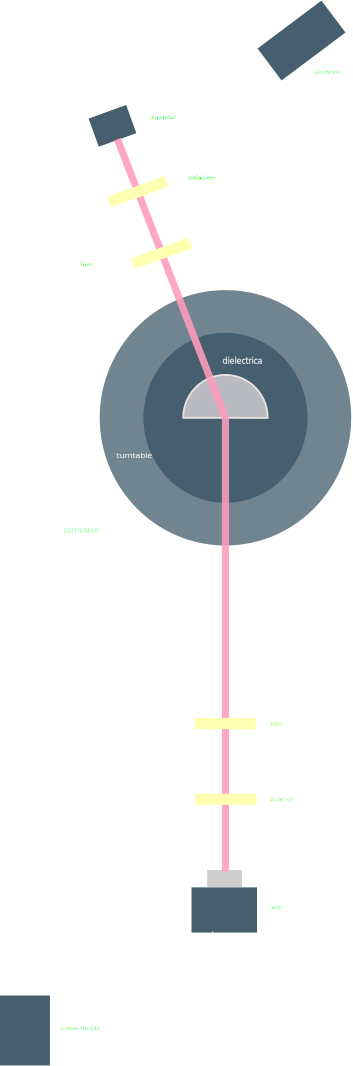
\includegraphics[width=1.1\textwidth]{figures/setup}
	\caption{Illustration of the setup.}
\end{marginfigure}
		For this experiment, we took great care in setting up the interferometer correctly, as the quality of our data relied solely on this. The (632 nm) laser initially strikes two mirrors, which are used to direct it and correct it horizontally. It then strikes the beam splitter, which is aligned perpendicularly to the ray. The light is then split in two beams of equal intensity. One is transmitted while the other is reflected. These beams then strike mirrors, which send them back towards the beam splitter, where they are gathered and directed towards a detector. Before striking the detector, they pass through a concave lens. This spreads the light more evenly over the sensors in the detector. On one of the mirrors, is mounted a piezoelectric element. Applying a voltage over this element allows us to vary the path distance as the piezoelectric expands and contracts. Lastly, we have placed the density filter in front of one of the mirrors. This allows us to gradualy change the intensity in one of the beams.
\section*{Results}
\subsection*{Piezo}
In our experiment we measure the induced voltage in the detector as a function of the changing potential over a piezoelectric element. We are interested in relating this changing voltage to the phase change, and thereby ultimately to the path change. In order to figure out how. As the piezoelectric, behaves differently for increasing and decreasing voltage have split our data accordingly. For both datasets, we have fit our data to functions of the form,
\[
	I_{E /C} \left( V \right) = A \cos \left( B + \Delta \rho_{E /C}\left( V \right)  \right) +D
.\] 
Where $A$ represents the amplitude of the measured signal and $B, D$ are constant offsets. We have found that,
\[
\delta \rho \left( V \right) = aV^{-kV}
\] makes for a description makes for a good description. We are not interested in examining how the detector converts light intensity to signal. We merely check that a constant $A$ is a good description of the fit. We are instead interested in checking whether the base $\cos\left( \Delta \rho  \right) $ is a good description of the data. Fig \textbf{4} and \textbf{5} contain examples of some data. We refrain from displaying all of our data. The results presented in the figure are quite representative of all our data.

\begin{marginfigure}[-450pt]
	\includegraphics[width=1.1\textwidth]{../example_contract}
	\caption{Data obtained from measuring the signal as the piezo-element is driven with linealy changing potential. The data has been sorted, leaving only the points pertaining to piezo-contraction.}
\end{marginfigure}
\begin{marginfigure}[-250pt]
	\includegraphics[width=1.1\textwidth]{../Piezo-expansion}
	\caption{Data obtained from piezo-contraction}
\end{marginfigure}
For each dataset, we make note of the estimated coefficients for $a$ and $k$. Fig  \textbf{6} is a plot of one of these functions. 
\begin{marginfigure}[-100pt]
	\includegraphics[width=1.1\textwidth]{figures/comparison}
	\caption{Comparison of our estimated function for the piezo-element to the theoretical function determined from the spec-sheet. In this case we have estimated $a_E = 1.7 \cdot 10^{-8}$, $k_E = 0.002$,  $a_C = 1.9 \cdot 10^{-8}$, $k_C = 0.004$}
\end{marginfigure}
\subsection*{Density filter}
We have measured the induced signal for varying degrees on the density filter. We have then used the amplitude of the measured wave as an estimate for the transmission-coefficient of the given angle. We have done this by normalizing the data at $\theta = 55$, we have set this value equal to the value from the spec-sheet. We have then scaled the rest of our data points in the same way. Remember, that the changing transmission-coefficient should in theory be the only factor impacting the intensity of the induced signal. Fig \textbf{7} shows our data, which seems to lie systematically below the data. The error is very small so it is not visible on the graph.
\begin{marginfigure}[-10pt]
	\includegraphics[width=1.1\textwidth]{../transmission}
	\caption{Comparison between measured transmission coefficients and one obtained from the density filter spec-sheet.}
\end{marginfigure}
\section*{Discussion}
We shall now examine our results more thoroughly, and try to determine why and how our data deviates from the expected results. In the experiment with the Piezo-element we examined the relationship between the displacement and the applied voltage:
\[
\Delta s \left( V \right)  = aV e^{-kV}
\]
By the use of CAS and the Piezo-element graph (\textbf{Figure 3}) given by ThorLab, the theoretical values was found to be:
\begin{center}

\textbf{Contraction: }[$k_C = 2.81\cdot 10^{-3}$,  $a_C = 2.68 \cdot 10^{-8}$], 
\\
\textbf{Expansion: }[$k_E = 1.40 \cdot 10^{-3}$, $a_E = 2.14 \cdot 10^{-8}$].
\end{center}
Using the error of 15 \% in the maximum displacement   as an estimate for the error in the Piezo-element we can fit the experimental data to the function. Using the same data from the comparison graph we found:
\begin{center}
\textbf{Contraction: }[$k_C = 4\cdot 10^{-3} \pm 0.11 \cdot 10^{-3}$,  $a_C = 1.9 \cdot 10^{-8} \pm 0.036 \cdot 10^{-8}$], 
\\
\textbf{Expansion: }[$k_E = 2 \cdot 10^{-3} \pm 0.13 \cdot 10^{-3}$, $a_E = 1.7 \cdot 10^{-8} \pm 0.038 \cdot 10^{-8}$].
\end{center}

It is clear that there is an offset present in the data because the fit is quite good with a low error but there is a visible difference compared to the theoretical fit. Both coefficients in the contradiction and expansion have a notable difference compared to the theoretical ones and our data yields a lower value for both slopes, which means the Piezo-element is not expanding and contracting as much as expected. It is hard to tell where this error comes from but an error that affected the interference pattern in the detector and thereby the path difference in the experiment is the vibrations and noise coming from the surroundings. It was clear that when the beams was nicely interfering in the detector a small disturbance coming from movement or people speaking could change the interference pattern. So ideally if the experiment was conducted in a more isolated area one would possibly get better results. Also one could expect the mirror connected to the Piezo-element to have an impact in how easy it was for the element to expand and contract.
\medskip

In the experiment with the density filter we wanted to examine the transmission coefficient given by  Thorlab:
\[
\beta(\theta)=10^{-0.00741\cdot \theta}
\]
Since the intensity is depended on the transmission coefficient and considering that the only thing we changed between measurements was the angle on the filter, a good estimate for measuring the transmission coefficient was to relate the change in the amplitude of the signal directly to the transmission coefficient, so dividing the maximum amplitude with the current one. We could then fit to the function:
\[
\beta(\theta)=10^{-a\cdot \theta}
\]
When fitting, the most obvious error was the one related to the measurement of the angle, where $\pm$ $0.5^{\circ}$ was a reasonable estimate. The fitting resulted in 
\begin{center}
[$a=1.1254 \pm 0.0661$]
\end{center}
Compared to the constant given by the manufacturer which was 0.00741, there is a big difference. Our measurements suffer from a systematic error, they lie beneath the expected curve and may even seem to follow a more exponential relation. The fit is pretty good though with a small error, so seems either we have a large contributing error or the relation given by the manufacturer may not be exact. \\
This systematic error is closely related to the angle on the filter wheel and it actually turns out that if the data is normalized around 20 degrees instead of 55 the fit gets much better with 
\begin{center}
$[a=0.4432 \pm 0.043$].
\end{center}
 We do not exactly know the reason for this angle error. We might have used the device wrongly or there might be a contributing error in our code. This does though still indicate that there is a mismatch with the constant given by ThorLabs because the transmission constant seems to be decreasing more rapidly and looks more exponential. 
 \\
There are other potential reasons that our data does not fit exactly. We have assumed that the detector converts intensity to signal with a linear function, and the data does seem to suggest this. If however, it is not exactly linear, it would lead to some systematic error. We have also assumed that opening the aperture on the detector would yield a constant scaling of the signal measured. This could again lead to a systematic error, as we opened the aperture once while taking data. 
\\
Both experiments yielded good fits but also a constant offset, which may indicate a systematic error in either some of the equipment or the code used for the data analysis, so a repetition of the experiment should be considered.
\section*{Conclusion}
In this experiment, we have pretty clearly seen that a wave-description of light is accurate. Michelson-morley setup does produce a sinusoidally varying intensity, this much we can say with certainty. Our data is definitely sinusoidal. We can also say with certainty, that the Piezo-element does note expand and contract identically. We found that the expansion and contraction coefficients were significantly different. So, broadly speaking, the experiment was succesful. However, if we were to use this setup, as quality assurance of the Piezo-element, we would have to improve it. There were to many uncertainties to conclude anything so specific.
\printbibliography
\end{document}
